% !TEX encoding = UTF-8
% !TEX TS-program = pdflatex
% !TEX root = ../tesi.tex

%**************************************************************
\chapter{Progettazione e implementazione}
\label{cap:progettazione-codifica}
%**************************************************************

\intro{Breve introduzione al capitolo}\\

%**************************************************************
\section{Prima versione smart contract}

La prima implementazione dello smart contract prevede l'utilizzo di due struct: Person e Contact

\begin{lstlisting}[language=Solidity]
    struct Person {
        string id;
        address owner;
        bool infected;
    }
\end{lstlisting}
\begin{lstlisting}[language=Solidity]
    struct Contact{
        Person p1;
        Person p2;
        uint256 contactRate;
        uint256 timestamp;
    }
\end{lstlisting}

I campi dati utilizzati dal contract sono i seguenti:
\begin{lstlisting}[language=Solidity]
contract Tracing {
    
    address ownerAddress;
    Person[] people;
    Contact[] contacts;

\end{lstlisting}
Al momento del deploy del contratto, ownerContract viene inizializzato con l’address appartenente a chi effettua il deploy.
I due array people e contacts, invece, vengono popolati in seguito.
People contiene tutte le persone che utilizzano lo smart contract, mentre contacts contiene tutti i contatti registrati tra due persone.\\
Non entrerò nel dettaglio del funzionamento di questo contract in quanto è stato scartato per favorire un’altra soluzione. Le ragioni risiedono in alcune criticità di questa implementazione. Avere una struttura dati che contiene tutti i contatti di tutti gli utenti non è una soluzione particolarmente furba. Per prima cosa complica inutilmente il contract per effettuare qualsiasi tipo di operazione sui contatti. In secondo luogo per il suo funzionamente sono richieste operazioni particolarmente onerose per quanto riguarda il consumo di gas, come il confronto tra stringhe. Infatti in solidity non è supportato il confronto booleano tra due stringhe. Per bypassare questo problema è necessario calcolare l’hash delle due stringhe e poi confrontarlo. Il calcolo dell’hash, però, è una delle operazioni più onerose in solidity.\\
Nella sezione analisi gas approfondirò l’argomento, mostrando i consumi del contract v1 a confronto con la soluzione definitiva.

\section{Seconda versione smart contract}
Come per la precedente soluzione sono stati adottati due struct, Person e Contact, ma con alcune differenze

\begin{lstlisting}[language=Solidity]
    struct Person {
        address owner;
        bool infected;
    }
\end{lstlisting}
\begin{lstlisting}[language=Solidity]
    struct Contact {
        string idContact;
        uint256 contactRate;
        uint256 timestamp;
    }
\end{lstlisting}
Person è una struct che ha come campi dati un address owner e un booleano infected.
Owner rappresenta l’address della persona. Infected invece, rappresenta lo stato di salute.
Contact è una struct che ha come campi dati una stringa idContact, un intero contactRate e un intero timestamp. IdContact rappresenta l’id della persona con cui si è entrati in contatto, contactRate è un indice di contatto tra le due persone e timestamp contiene l’unix time del momento del contatto.\\

I campi dati sono i seguenti:
\begin{lstlisting}[language=Solidity]
contract Tracing {
    
    address ownerAddress;
    mapping(string => Person) mapIdToPerson;
    mapping(string => Contact[]) mapIdToContact;

\end{lstlisting}
Lo smart contract possiede un campo address ownerContract che rappresenta il proprietario del contratto.
Al momento del deploy ownerContract viene inizializzato all’address appartenente a chi effettua il deploy.
mapIdToPerson associa un id ad una persona. La mappa contiene tutte le persone che utilizzano il contract. 
mapIdToContact associa un id ad un array di contatti. Ogni array rappresenta i contatti della persona con il corrispondente id.\\

Le funzioni disposibili per un uso esterno nel contract sono le seguenti:
\begin{lstlisting}[language=Solidity]
/*
Add a person in mapIdToPerson
If the person is already in, returns an error
*/
function addPerson(string calladata _id, address _owner) external;

/*
Change the state of infected for the person of the input id
Returns an error if the id isn't registered or if there aren't the permission to call the function: only the owner of the contract can call this function.
*/    
function setInfected(string calladata _id,bool _infected) external;

/*
Return the infected state of a person
Returns an error if the call is from a user without permission or if the id isn't registered
*/
function getInfected(string calladata _myId,string calladata _idContact) external view isOwner(_myId) returns (bool);

/*
Adds a contact in mapIdToContacts
Returns an error if one of the ids doesn't exists
*/    
function addContact(string calladata _myId,string calladata _idContact,uint _contactRate) external isOwner(_myId);

/*
Returns an array of id contacts of the person.
*/    
function getContactsById(string calladata _id) external view returns(string[] memory);

/*
Check if in the contacts of a person there are people infected
Returns an error if the call is from a user without permission
*/    
function hasIdHadRiskyContacts(string calladata _id,uint _contactRate,uint _days) external view isOwner(_id) returns (bool);

/*
Sums a person contactRates in the last days
Returns an error if the call is from a user without permission
*/   
function sumContactRate(string calladata _id,uint256 _days) external view isOwner(_id) returns (uint256);
\end{lstlisting}

\section{Analisi gas}
In ethereum ogni operazione effettuata che cambia lo stato della blockchain consuma gas. Il gas è un’unità di misura utilizzata per pagare la computazione effettuata dai miners. Più un operazione è dispendiosa a livello di risorse, più gas questa operazione costerà.
Il concetto di gas permette di addebitare una tariffa che viene pagata ai miners, incentivandoli a prendere parte attiva nel sistema ethereum.
Tuttavia, il gas rappresenta un cambio di paradigma rispetto alla programmazione classica. Non sempre un approccio vantaggioso in un normale linguaggio di programmazione rappresenta la best practice in solidity, proprio perché c’è una variabile in più da considerare. 
Nel corso dello stage è stata rivolta particolare attenzione a questo aspetto: sono state portate modifiche molto importanti al contract definitivo per ottimizzare il più possibile il consumo di gas.\\

Nei paragrafi precedenti ho mostrato la prima implementazione scartata per un eccessivo consumo di gas. Qui sotto riporto i costi relativi alle due versioni.

\begin{figure}[h]
\caption{Primo smart contract}
\centering
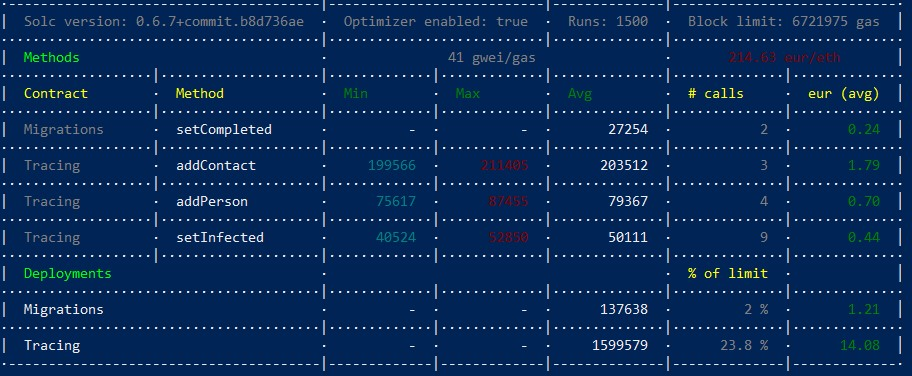
\includegraphics[width=1.0\textwidth]{./immagini/costiTracingOptimizer}
\end{figure}

\begin{figure}[h]
\caption{Secondo smart contract}
\centering
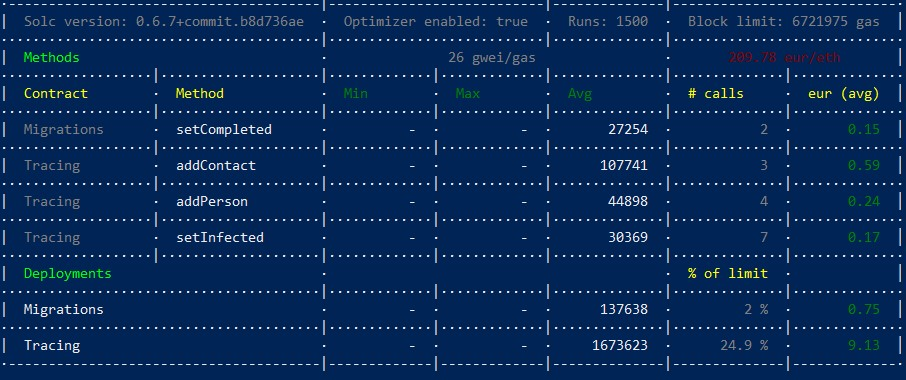
\includegraphics[width=1.0\textwidth]{./immagini/nuoviCosti}
\end{figure}

Il costo del deploy del deploy dei due smart contracts è abbastanza simile: intorno a 1.500.000 gas. Questo però non rappresenta il costo maggiore per quanto riguarda l’applicazione di contact tracing. 
Il deploy infatti, viene effettuato una singola volta e il suo costo rimane marginale.
La parte più onerosa è certamente il consumo che riguarda le funzioni addPerson, addContact e setInfected.
Si può notare che per ogni chiamata di queste funzioni il consumo di gas è all’incirca dimezzato.
\begin{itemize}
\item{addContact: 200k prima, 100k dopo}
\item{addPerson: 80k prima, 45k dopo}
\item{setInfected: 50k prima, 30k dopo}
\end{itemize}

\subsection{Fattibilità applicazione reale}
Anche con la massima efficienza di uno smart contract, è fondamentale considerare il caso d’uso dell’applicazione per rendersi conto della fattibilità del progetto.
Come accennato prima, i costi maggiori in ethereum non sono rappresentati dal deploy del contratto, bensì dal numero di chiamate stimate alle funzioni che consumano gas.
Nel nostro caso d’uso la funzione addPerson viene eseguita ogni qualvolta una persona installa l’applicazione nel proprio smartphone. Considerando metà della popolazione italiana questo vuol dire 30 milioni di chiamate. Prendendo come esempio di prezzo per gas 26 gwei, ogni chiamata costa circa 24 centesimi. Questo vuol dire che sono per l’installazione il costo stimato è di 7,5 milioni di euro.
Già questo piccolo calcolo sarebbe sufficiente per rendersi conto che questo smart contract non è sostenibile in un contesto di utilizzo reale. Purtroppo però, c’è una spesa ancora maggiore. In blockchain viene inserito ogni contatto superiore a 15 minuti a distanza inferiore di 2 metri, per ogni persona che ha l’applicazione. Facendo una piccola stima, se consideriamo una media di 10 contatti di questo tipo a persona al giorno, con ogni chiamata di costo pari a 0,50 centesimi circa, si ottiene una spesa di ben 150 milioni di euro (al giorno!).
Decisamente non sostenibile. Soluzioni di questo genere non sono realizzabili e questo smart contract rappresenta un lavoro puramente accademico, senza alcuna possibilità di utilizzo reale. 
Tuttavia ci sono delle soluzioni alternative.
\\
\subsection{Soluzioni}
\subsubsection{Smart contract semplificato}
Come detto, in ethereum la soluzione proposta non è realizzabile nella pratica. Una possibile alternativa nell’ambito contact tracing è rappresentata dalla gestione locale di tutti i contatti tra le persone. Ogni dispositivo mobile possiede un id e i contatti con gli altri dispositivi (distanza inferiore a 2 metri per almeno 15 minuti) vengono registrati e salvati localmente. Ogni 14 giorni vengono eliminati perché considerati ininfluenti per il contagio.
Quando una persona viene trovata infetta a seguito di un tampone, il medico (sotto autorizzazione del contagiato) lo segnala tramite web app. Quello che succede in seguito a questa segnalazione è che l’id del malato viene inserito nell’array degli infetti nello smart contract. 
Lato mobile periodicamente il dispositivo chiama una funzione dello smart contract che restituisce gli infetti degli ultimi 14 giorni. In seguito controlla se tra i suoi contatti è presente un infetto o meno.
In questo modo lo smart contract è estremamente semplice e si occupa solo di conservare gli id dei malati in modo sicuro e immutabile.
Tutte le altre operazioni sono effettuate localmente. Il consumo del gas è infinitamente più contenuto e permette un utilizzo reale dell’applicazione. Inoltre non sono presenti rallentamenti dovuti ai tempi di validazione delle transazioni. Questo perché l’unica operazione che richiede consumo di gas, e dunque una transazione, è quella di inserimento dell’id nell’array, che viene effettuata dal medico solo per le persone malate a seguito di un tampone positivo. Questa operazione non è necessario che sia immediata, ma può senza problemi impiegare il tempo necessario per la validazione in una blockchain. Dal lato mobile infatti, il controllo di infetti presenti tra i contatti non è real-time, ma viene effettuato periodicamente.
Le funzioni presenti in questo smart contract sono solo due: una per l’inserimento di un infetto, l’altra per ottenere la lista di infetti. Quest’ultima non richiede una transazione in quanto è una funzione di sola lettura.\\

\begin{figure}[h]
\caption{Nuovo smart contract}
\centering
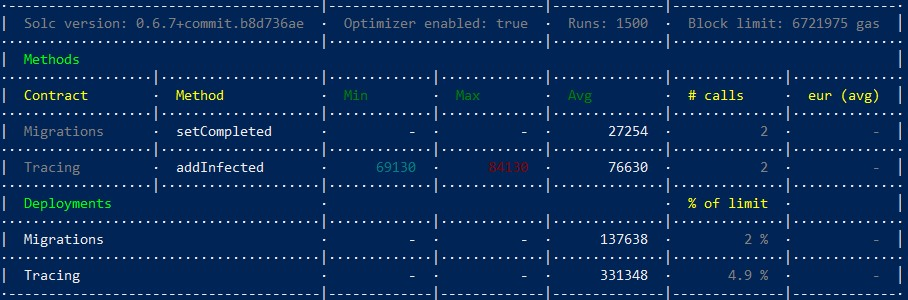
\includegraphics[width=1.0\textwidth]{./immagini/costiOnlyInfected}
\end{figure}

Dalla tabella riportata si può notare come il costo di deploy del contratto sia notevolmente inferiore rispetto ai precedenti contratti: 300k gas contro 1500k circa. 
Ma la differenza la fa soprattutto il numero di chiamate alla funzione addInfected, decisamente inferiori rispetto a tutte le chiamate necessarie per registrare i contatti.
In Italia i contagi certificati ad oggi sono circa 200k. Considerando un costo di circa 20 centesimi a chiamata per ogni infetto, supponendo anche che tutti gli infetti siano registrati all’applicazione e diano il consenso al proprio medico, la spesa totale dell’utilizzo del contratto si aggirerebbe intorno a 40k euro, in linea con le dApp più utilizzate. \\
\subsubsection{Altre blockchain}
Un’altra soluzione, che può essere anche complementare a quella appena descritta, prevede un cambio di piattaforma. Ethereum infatti, nonostante sia la blockchain più diffusa per lo sviluppo di applicazioni decentralizzate, ha un costo molto alto e destinato ad aumentare con l’aumentare degli utenti.
Questo è dovuto all’algoritmo di consenso che ethereum, come la maggiorparte delle blockchain, utilizza attualmente, ossia il proof of work. La computazione richiesta per validare i blocchi e le transazioni richiedono il pagamento di una tassa, proporzionale alle risorse richieste. 
Tuttavia, esistono altri tipi di blockchain che utilizzano il consenso proof of stake, come la piattaforma EOS.
La scalabilità e le transazioni gratuite sono i punti di forza di EOS. Il processo non è comunque gratuito, ma richiede che l’utente possieda un numero di token (stake) che gli permetta di “affittare” le risorse necessarie per validare le transazioni. Questi token però non sono spesi, ma possono essere restituiti quando si vuole al prezzo corrente della cryptovaluta.
Anche ethereum sta effettuando il passaggio al proof of stake, con la piattaforma che verrà denominata ethereum 2.0, in arrivo a fine 2020. 
Il passaggio definitivo, con la chiusura di ethereum 1.0 è previsto per il 2022.
Ethereum 2.0 è molto atteso perché il cambio di algoritmo cambia completamente il modo di vedere le blockchain. La scalabilità è uno dei problemi maggiori delle blockchain che si basano su proof of work, limitandone le possibilità di applicazione. Invece con EOS ora e con ethereum 2.0 nel futuro sarà possibile utilizzare le blockchain per qualsiasi tipo di applicazione decentralizzata senza accusare differenze rispetto a una tradizionale applicazione.

\section{Test smart contract}
I test dello smart contract sono stati fatti con il linguaggio JavaScript sfruttando la suite truffle.
Di seguito è riportata la tabella di tracciamento dei test.

\renewcommand{\arraystretch}{3}
\begin{center}
	\begin{longtable}{| c | p{25em} | c |}
		\caption{Tabella test smart contracti}
		\label{tab:test-sci}\\
		\hline
		\textbf{Test id} & \centering\textbf{Descrizione} & \textbf{Requisiti coperti}\\
		\endfirsthead
		\hline
		\textbf{Test id} & \centering\textbf{Descrizione} & \textbf{Requisiti coperti}\\
		\endhead
		\endfoot
		
		\hline
		UT-1     & Should deploy smart contract properly and save owner address & RFN-1 \\
		\hline
		UT-2     & Should add two person to people array and get them by id & RFN-2 - RF10\\
		\hline
		UT-3     & Should not be able to add the same id person in people array & RFN-3 \\
		\hline
		UT-4     & Should add a contact between two id presents in people array & RFN-7 \\
		\hline
		UT-5     & Should not be able to add another person contacts & RFN-8 \\
		\hline
		UT-6     & Should not be able to add a contact with nonexisting person & RFN-9 \\
		\hline
		UT-7     & Should set a person infected & RFN-4 \\
		\hline
		UT-8     & Should not be able to set a person infected if the address is not who deploy the contract & RFN-5 \\
		\hline
		UT-9     & Should not be able to set infected a nonexisting person & RFN-6 \\
		\hline
		UT-10   & Should not be able to get other people contacts & RFN-11 \\
		\hline
		UT-11   & Should check that the second id has a infection risk & RFN-12 \\
		\hline
		UT-12   & Should check that if a contact is not confirmed, then a person has not risk infection &  13\\
		\hline
		UT-13   & Should not be able to check another person risk infection & RFN-14 \\
		\hline
		UT-14   & Should check that sum of contactRates in the last day is 15 for the first id & RFN-15 \\
		\hline
		UT-15   & Should not be able to calculate another person sum of contactRates & RFN-16 \\
		\hline
	\end{longtable}
\end{center}

\chapter{Integrazione in applicazione di contact tracing}

\section{Applicazione android}

\subsection{Requisiti}
\begin{enumerate}
	\item{Smart contract Tracing.sol}
	\item{Address contratto}
	\item{Chiave privata wallet}
	\item{Address wallet}
	\item{Compilatore solc}
	\item{Web3j}
	\item{Android studio}
\end{enumerate}

\subsection{Installazione}
Scaricare web3j dalla repo su \href{https://github.com/web3j/web3j/releases}{Github}\\\
Estrarre lo zip scaricato con il seguente
\begin{lstlisting}[numbers=none]
	unzip web3j-<version>.zip
\end{lstlisting}
Eseguire web3j con 
\begin{lstlisting}[numbers=none]
	web3j-<version>/bin/web3j
\end{lstlisting}
Creare i file .abi e .bin dello smart contract con il comando
\begin{lstlisting}[numbers=none]
	solcjs ./Tracing.sol --bin --abi --optimize -o ./ 
\end{lstlisting}
A partire dai file .bin e .abi generare la classe java
\begin{lstlisting}[numbers=none]
	web3j solidity generate -b ./Tracing.bin -a ./Tracing.abi -o ./ -p GeneratedClasses 
\end{lstlisting}
In questo modo nella directory /GeneratedClasses si troverà la classe Tracing.java, da inserire nel progetto di android per permettere l'integrazione dell'app con la blockchain.
L'ultimo passaggio da effettuare per interagire con il contract è includere nel file build.gradle la dipendenza con la libreria web3j, inserendo la seguente riga
\begin{lstlisting}[numbers=none]
	implementation'org.web3j:core:<version>' 
\end{lstlisting}

\subsection{Utilizzo smart contract}
Per utilizzare lo smart contract è stata creata la classe BlockchainManager che si occupa di caricare il contratto, creare delle credenziali e gestirne le funzioni.
Di seguito viene riportata la classe sviluppata:
\begin{lstlisting}[language = Java]
import android.content.Context
import android.util.Log
import androidx.preference.PreferenceManager
import com.google.gson.Gson
import it.synclab.synctrace.mobile.tracinglib.db.User
import org.bouncycastle.jce.provider.BouncyCastleProvider
import org.web3j.crypto.Credentials
import org.web3j.crypto.Keys
import org.web3j.crypto.Wallet
import org.web3j.protocol.Web3j
import org.web3j.protocol.core.DefaultBlockParameterName
import org.web3j.protocol.http.HttpService
import org.web3j.tx.Transfer
import org.web3j.utils.Convert
import java.math.BigDecimal
import java.math.BigInteger
import java.security.Security

class BlockchainManager {

    companion object {
        private const val TAG = "BlockchainManager"
        private val GAS_LIMIT = BigInteger.valueOf(6721975L)
        private val GAS_PRICE = BigInteger.valueOf(20000000000L)
		//private key metamask account
        private const val PRIVATE_KEY = YOUR_PRIVATE_KEY
		//address del contract
        private const val CONTRACT_ADDRESS = ADDRESS
        // shared preferences keys
        private const val CREDENTIALS = "bc_credentials"
        private const val TRANSACTION_CREDENTIALS = "bc_transaction_credentials"
    }

    private val web3j = Web3j.build(HttpService(
        "https://ropsten.infura.io/v3/YOUR_INFURA_ID"
    ))

    init {
        setupBouncyCastle()
    }

    private fun setupBouncyCastle() {
        val provider =
            Security.getProvider(BouncyCastleProvider.PROVIDER_NAME)
                ?: 
                return
        if (provider.javaClass == BouncyCastleProvider::class.java) {
            return
        }
        Security.removeProvider(BouncyCastleProvider.PROVIDER_NAME)
        Security.insertProviderAt(BouncyCastleProvider(), 1)
    }

    fun registerPersonIfFirstTime(context: Context) {
        if (!areCredentialsPresent(context)) {
            val transactionCredentials = Credentials.create(PRIVATE_KEY)
            // create new private/public key pair
            val keys = Keys.createEcKeyPair()
            val uuid = User.getUuid(context)
            val wallet = Wallet.createLight(uuid, keys)
            val credentials = Credentials.create(Wallet.decrypt(uuid, wallet))

            sendFunds(context, 0.2, credentials, transactionCredentials)

            try {
                val tracingContract = loadContract(context, credentials)
                tracingContract.addPerson(uuid, credentials.address).sendAsync().get()
            } catch (e: Exception) {
                Log.e(TAG, "Cannot add person", e)
                return
            }

            setCredentials(context, credentials, transactionCredentials)
            Log.i(TAG, "Created credentials and registered person")
        }
    }

    private fun areCredentialsPresent(context: Context): Boolean {
        val sp = PreferenceManager.getDefaultSharedPreferences(context)
        return sp.getString(CREDENTIALS, null) != null
    }

    private fun getCredentials(context: Context): Credentials {
        val sp = PreferenceManager.getDefaultSharedPreferences(context)
        val jsonCredentials = sp.getString(CREDENTIALS, null)
        return Gson().fromJson(jsonCredentials, Credentials::class.java)
    }

    private fun getTransactionCredentials(context: Context): Credentials {
        val sp = PreferenceManager.getDefaultSharedPreferences(context)
        val jsonCredentials = sp.getString(TRANSACTION_CREDENTIALS, null)
        return Gson().fromJson(jsonCredentials, Credentials::class.java)
    }

    private fun setCredentials(context: Context, credentials: Credentials,
                               transactionCredentials: Credentials) {
        val sp = PreferenceManager.getDefaultSharedPreferences(context)
        val gson = Gson()
        sp.edit().apply() {
            putString(CREDENTIALS, gson.toJson(credentials))
            putString(TRANSACTION_CREDENTIALS, gson.toJson(transactionCredentials))
        }.apply()
    }

    private fun loadContract(context: Context, credentials: Credentials = getCredentials(context)): TracingContract {
        return TracingContract.load(CONTRACT_ADDRESS, web3j, credentials, GAS_PRICE, GAS_LIMIT)
    }

    private fun sendFunds(context: Context, amount: Double,
                          credentials: Credentials = getCredentials(context),
                          transactionCredentials: Credentials = getTransactionCredentials(context)) {
        try {
            Transfer.sendFunds(
                web3j, transactionCredentials, credentials.address,
                BigDecimal.valueOf(amount), Convert.Unit.ETHER
            ).sendAsync().get()
        } catch (e: Exception) {
            Log.e(TAG, "Cannot send funds", e)
        }
    }

    fun addContact(context: Context, myUuid: String, contactUuid: String, contactIndex: Double) {
        try {
            val tracingContract = loadContract(context)
            tracingContract.addContact(myUuid, contactUuid, BigInteger.valueOf(contactIndex.toLong()))
                .sendAsync().get()

            val ethGetBalance =
                web3j.ethGetBalance(CONTRACT_ADDRESS, DefaultBlockParameterName.LATEST).sendAsync().get()
            val wei = ethGetBalance!!.balance
            if (wei.compareTo(BigInteger.valueOf(100000000000000000L)) == -1) {
                sendFunds(context, 0.1)
            }
        } catch (e: Exception) {
            Log.e(TAG, "Cannot add contact to blockchain", e)
        }
    }
}

\end{lstlisting} 

In questa classe per effettuare le chiamate alle funzioni dello smart contract è sufficiente richiamare la funzione seguita da una chiamata asincrona, come per il seguente caso:

\begin{lstlisting}[numbers=none]
	tracingContract.addPerson(
		uuid,credentials.address
	).sendAsync().get()
\end{lstlisting}
Grazie a questa classe che gestisce il contratto, nell'applicazione è possibile utilizzare le funzioni dello smart contract dove desiderato.

\section{Web application}
\subsection{Requisiti}
\begin{itemize}
	\item{Node.js}
	\item{Address contratto}
	\item{Chiave privata wallet}
	\item{Address wallet}
\end{itemize}
\subsection{Utilizzo smart contract}
Per interagire con lo smart contract dalla web application è stato utilizzato uno script opportunamente inserito nel codice dell'applicazione.
Questo script permette di effettuare una chiamata alla funzione setInfected dello smart contract. SetInfected viene richiamata solo nella web application in quanto è autorizzato a effettuare la chiamata solo il personale medico. Per accertarsi di questo anche nello smart contract, la funzione può essere chiamata solo dall'address di chi fa il deploy del contract. Per questo l'address che fa la chiamata nello script (salvato nella variabile addressFrom) è lo stesso indirizzo di chi fa il deploy.\\\\
Quando dalla schermata in figura 5.1 un medico inserisce un infetto, viene effettuata una chiamata alla relativa funzione nello smart contract.

\begin{figure}[h]
\caption{Inserimento infetti da web application}
\centering
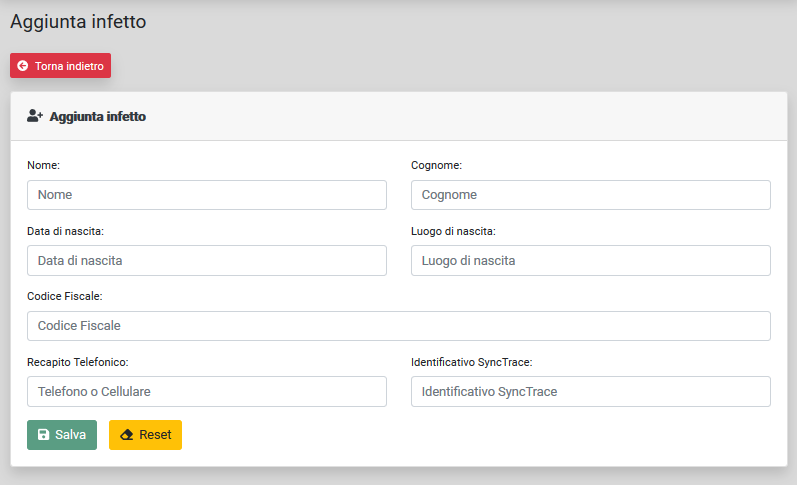
\includegraphics[width=1.0\textwidth]{./immagini/webapp_infected}
\end{figure}

Lo script utilizzato per farlo è il seguente:
\begin{lstlisting}
const Web3 = require('web3')
Tx = require("ethereumjs-tx").Transaction

// connect to Infura node
const web3 = new Web3(new Web3.providers.HttpProvider('https://ropsten.infura.io/v3/YOUR_INFURA_ID'))

// the address that will send the test transaction
const addressFrom = 'YOUR_METAMASK_ADDRESS'
//private key of metamask account, be aware of the security
const privKey = environment.BC_PRIVATE_KEY;

// the contract address
const addressTo = 'CONTRACT_ADDRESS'

//abi of the contract
const abi = 'CONTRACT_ABI'

// Signs the given transaction data and sends it. Abstracts some of the details 
// of buffering and serializing the transaction for web3.
function sendSigned(txData, cb) {
  const privateKey = Buffer.from(privKey, 'hex')
  const transaction = new Tx(txData, {'chain':'ropsten'})
  transaction.sign(privateKey)
  const serializedTx = transaction.serialize().toString('hex')
  web3.eth.sendSignedTransaction('0x' + serializedTx, cb)
}

const myContract = new web3.eth.Contract(JSON.parse(abi), addressTo);

const myData = myContract.methods.setInfected( INFECTED_ID,true).encodeABI();

// get the number of transactions sent so far so we can create a fresh nonce
web3.eth.getTransactionCount(addressFrom).then(txCount => {

  // construct the transaction data
  const txData = {
    nonce: web3.utils.toHex(txCount),
    gasLimit: web3.utils.toHex(6721975),
    gasPrice: web3.utils.toHex(20000000000), 
    to: addressTo,
    from: addressFrom,
    value: web3.utils.toHex(web3.utils.toWei("0", 'wei')),
    data: myData 
  }

  // fire away!
  sendSigned(txData, function(err, result) {
    if (err) return console.log('error', err)
    console.log('sent', result)
  })

})

\end{lstlisting}
